% ============================================================
% Beamer — ISLP Lecture Series — IMPROVED EDITION
% Advanced Module A1: Randomised Controlled Trials
% ============================================================
\documentclass[aspectratio=169,11pt]{beamer}
\usepackage[utf8]{inputenc}\usepackage[T1]{fontenc}\usepackage[english]{babel}
\usepackage{graphicx}\usepackage{booktabs}\usepackage{amsmath,amssymb,amsfonts}
\usepackage{mathtools}\usepackage{hyperref}\usepackage{xcolor}
\usepackage{verbatim}\usepackage{alltt}
\usepackage{tikz}\usetikzlibrary{calc,arrows.meta,positioning,shapes}
\usepackage{tcolorbox}\tcbuselibrary{skins}

\usetheme{Madrid}\usecolortheme{default}
\setbeamertemplate{navigation symbols}{}
\setbeamertemplate{footline}[frame number]
\setbeamertemplate{blocks}[rounded][shadow=false]
\setbeamertemplate{headline}{%
  \leavevmode\hbox{%
    \begin{beamercolorbox}[wd=\paperwidth,ht=2.2ex,dp=0.9ex]{section in head/foot}%
      {\fontsize{4.6}{5.2}\selectfont%
       \insertsectionnavigationhorizontal{\paperwidth}{}{\hskip0pt plus1filll}}%
    \end{beamercolorbox}}%
}
\setbeamerfont{section in head/foot}{size=\tiny}
\setbeamerfont{palette primary}{size=\tiny}
\setbeamerfont{palette tertiary}{size=\tiny}
\setbeamerfont{section in toc}{size=\footnotesize}

\usepackage{listings}
\definecolor{pyKw}{RGB}{0,0,180}\definecolor{pyStr}{RGB}{20,120,40}
\definecolor{pyCom}{RGB}{120,120,120}\definecolor{accent}{RGB}{38,70,140}
\lstdefinestyle{Pystyle}{language=Python,basicstyle=\ttfamily\footnotesize,
  keywordstyle=\color{pyKw}\bfseries,commentstyle=\color{pyCom}\itshape,
  stringstyle=\color{pyStr},showstringspaces=false,upquote=true,
  columns=fullflexible,breaklines=true,literate={~}{{$\sim$}}1}
\lstset{style=Pystyle}

% Tighter TOC spacing (place AFTER \lstset, BEFORE \AtBeginSection)
\usepackage{etoolbox}
\makeatletter
\patchcmd{\beamer@sectionintoc}{\vskip1.5em}{\vskip.6em}{\typeout{TOCPATCH-OK}}{\typeout{TOCPATCH-FAIL}}
\makeatother

\AtBeginSection[]{\begin{frame}{Outline}\footnotesize
  \tableofcontents[currentsection,sectionstyle=show/shaded,subsectionstyle=show/show/hide]
\end{frame}}

\newcommand{\islpsource}[1]{%
  \vfill\hfill{\tiny\itshape\color{gray}Source: #1 \textemdash{} ISLP, James et al.\ (2023).}\par
}

\newtcolorbox{takeaway}[1][Takeaway]{enhanced,colback=green!4,colframe=green!50!black,
  boxrule=0pt,leftrule=2.5pt,arc=2pt,fonttitle=\bfseries,title=#1,
  left=2mm,right=2mm,top=1mm,bottom=1mm}
\newtcolorbox{numexample}[1][Worked example]{enhanced,colback=orange!4,colframe=orange!70!black,
  boxrule=0pt,leftrule=2.5pt,arc=2pt,fonttitle=\bfseries,title=#1,
  left=2mm,right=2mm,top=1mm,bottom=1mm}
\newtcolorbox{readme}[1][How to read this]{enhanced,colback=blue!4,colframe=accent,
  boxrule=0pt,leftrule=2.5pt,arc=2pt,fonttitle=\bfseries,title=#1,
  left=2mm,right=2mm,top=1mm,bottom=1mm}

\title{Quantitative Research Methods}
\subtitle{Randomised Controlled Trials\\[2pt]{\small Advanced module A1 --- optional self-study}}
\author{Prof.\ Dr.\ Christoph Weisser}
\date{}\graphicspath{{images/}}

\newtcolorbox{exercise}[1][Exercise]{enhanced, fontupper=\footnotesize, colback=purple!4, colframe=purple!55!black, boxrule=0pt, leftrule=2.5pt, arc=2pt, fonttitle=\bfseries, title=#1, left=2mm, right=2mm, top=1mm, bottom=1mm}
\newtcolorbox{solutionbox}[1][Solution]{enhanced, fontupper=\footnotesize, colback=teal!5, colframe=teal!55!black, boxrule=0pt, leftrule=2.5pt, arc=2pt, fonttitle=\bfseries, title=#1, left=2mm, right=2mm, top=1mm, bottom=1mm}
\newtcolorbox{longexercise}[1][Extended exercise (15 min)]{enhanced, fontupper=\footnotesize, colback=violet!6, colframe=violet!55!black, boxrule=0pt, leftrule=3pt, arc=2pt, fonttitle=\bfseries, title=#1, left=2mm, right=2mm, top=1mm, bottom=1mm}

% Reclaim ~2pt of body height (custom nav headline makes full slides tip over by ~1.83pt)
\addtobeamertemplate{frametitle}{}{\vspace{-2pt}}

\newtcolorbox{labnote}[1][Run this live in the lab notebook]{enhanced, fontupper=\footnotesize, colback=cyan!7, colframe=cyan!45!black, boxrule=0pt, leftrule=3pt, arc=2pt, fonttitle=\bfseries, title=#1, left=2mm, right=2mm, top=1mm, bottom=1mm}

% Industry application callout box --- slate grey, for real business/industry use
\definecolor{industryC}{RGB}{88,98,116}
\newtcolorbox{industry}[1][In industry]{enhanced, fontupper=\footnotesize, colback=industryC!7, colframe=industryC, boxrule=0pt, leftrule=3pt, arc=2pt, fonttitle=\bfseries, title={In industry --- #1}, left=2mm, right=2mm, top=1mm, bottom=1mm}

% Common-mistake callout --- crimson, for the error to pre-empt
\newtcolorbox{mistake}[1][Common mistake]{enhanced, fontupper=\footnotesize, colback=red!4, colframe=red!60!black, boxrule=0pt, leftrule=3pt, arc=2pt, fonttitle=\bfseries, title=#1, left=2mm, right=2mm, top=1mm, bottom=1mm}

\begin{document}
\begin{frame}[plain]\titlepage\end{frame}

\begin{frame}{Where this module fits}
  \footnotesize
  \begin{center}
  \begin{tabular}{@{}p{3.6cm}p{8.6cm}@{}}
    \toprule
    \textbf{Course chapter} & \textbf{What this module builds on it} \\
    \midrule
    Ch.\ 0 --- pre-course refresher & The two-sample $t$-test \emph{is} the basic RCT analysis \\
    Ch.\ 3 --- linear regression & Regression adjustment for precision; robust standard errors \\
    Ch.\ 4 --- classification & Binary outcomes (conversion) as experiment metrics \\
    Ch.\ 5 --- resampling & Simulated sampling distributions; power by simulation \\
    Ch.\ 13 --- multiple testing & Peeking and metric panels as multiplicity problems \\
    \bottomrule
  \end{tabular}
  \end{center}
  \vspace{2pt}
  \begin{takeaway}[A new question --- not a better model]
    Chapters 2--10 estimated $\hat f(x)\approx E[Y\mid X=x]$ --- \textbf{correlational} by
    design, and exactly right for prediction. This module asks the \textbf{interventional}
    question: what happens to $Y$ if \emph{we} set the treatment $D$? No amount of model
    flexibility answers it; different \emph{data} --- randomised data --- do.
  \end{takeaway}
  {\scriptsize One of four optional advanced modules; self-study, with a companion lab notebook.}
\end{frame}

\begin{frame}{Contents}\small\tableofcontents[hideallsubsections]
  \vfill
  {\tiny Optional and advanced material is collected in the \textbf{appendix} at the end of the deck.}
\end{frame}

\begin{frame}{Notation in this module}
  \footnotesize
  \begin{center}
  \begin{tabular}{@{}ll@{}}
    \toprule
    \textbf{Symbol} & \textbf{Meaning} \\
    \midrule
    $Y_i(1),\,Y_i(0)$ & potential outcomes of unit $i$ with / without treatment \\
    $D_i$ & treatment indicator ($1$ = treated); $Z_i$: \emph{assignment} when they differ \\
    $Y_i = D_iY_i(1)+(1-D_i)Y_i(0)$ & the observed outcome \\
    $\tau_i = Y_i(1)-Y_i(0)$ & individual treatment effect (ITE) \\
    $\tau = E[\tau_i]$ & average treatment effect (ATE) \\
    ATT, ATU & average effect on the treated / the untreated \\
    $\pi = \Pr(D_i=1)$ & share treated \\
    $n_1,\,n_0$; \ $\bar Y_1,\,\bar Y_0$ & arm sizes and arm means; $\hat\tau=\bar Y_1-\bar Y_0$ \\
    $S_1^2,\,S_0^2$ & sample variances within the arms \\
    $\sigma^2$ & outcome variance used in power planning \\
    $\delta$ & effect size to detect; MDE: minimum detectable effect \\
    $\alpha$, $1-\beta$ & two-sided test size and power; $z_q$: standard normal quantile \\
    $\rho$ & intraclass correlation within a cluster; DE: design effect \\
    $X_i$ & pre-treatment covariates \\
    \bottomrule
  \end{tabular}
  \end{center}
\end{frame}

\begin{frame}{Sources and references}
  \begin{block}{Primary textbook (course reference)}
    James, G., Witten, D., Hastie, T., Tibshirani, R., \& Taylor, J.\ (2023).
    \emph{An Introduction to Statistical Learning, with Applications in
    Python.} Springer.
  \end{block}
  \begin{block}{Foundations for this module}
    Neyman (1923); Rubin (1974) --- potential outcomes. \
    Imbens, G.\ \& Rubin, D.\ (2015). \emph{Causal Inference for Statistics, Social, and
    Biomedical Sciences.} Cambridge University Press. \
    Kohavi, R., Tang, D., \& Xu, Y.\ (2020). \emph{Trustworthy Online Controlled
    Experiments.} Cambridge University Press.
  \end{block}
\end{frame}

\begin{frame}{Learning objectives}
  By the end of this module you will be able to:
  \begin{itemize}
    \item \textbf{Explain} potential outcomes, the fundamental problem of causal
          inference, and SUTVA.
    \item \textbf{Derive} the selection-bias decomposition of a naive group comparison.
    \item \textbf{Analyse} a randomised experiment with the difference in means, the
          two-sample $t$-test, and regression adjustment with robust standard errors.
    \item \textbf{Design} an experiment: power, sample size, minimum detectable effect,
          stratified and cluster randomisation.
    \item \textbf{Recognise} the threats --- attrition, non-compliance, peeking --- and
          \textbf{apply} the intention-to-treat principle.
    \item \textbf{Frame} industrial A/B testing as the RCT it is.
  \end{itemize}
\end{frame}

\begin{frame}{Roadmap of this module}
  \begin{takeaway}[From correlation to causation]
    \begin{enumerate}
      \item Why prediction is not causation: a confounded training programme.
      \item Potential outcomes, estimands, SUTVA --- and the selection-bias decomposition.
      \item Randomisation: why it works; the difference-in-means estimator.
      \item Analysis in practice: regression adjustment, robust standard errors.
      \item Design: power, minimum detectable effect, blocking, clusters.
      \item Threats and practice: attrition, non-compliance, balance, peeking, A/B tests.
    \end{enumerate}
  \end{takeaway}
\end{frame}

\begin{frame}{Where this module is used in industry}
  \scriptsize
  \begin{center}
  \begin{tabular}{@{}p{2.9cm}p{5.2cm}p{4.4cm}@{}}
    \toprule
    \textbf{Sector} & \textbf{Concrete application} & \textbf{Which decision it drives} \\
    \midrule
    Tech, e-commerce & A/B tests on features, ranking, pricing UX & Ship or roll back the change \\
    Pharma & Phase-III randomised, double-blind trials & Whether the drug is approved \\
    Development, policy & Cash-transfer and nudge experiments & Which programme is scaled up \\
    Marketing & Incrementality / uplift tests with holdout groups & Where the ad budget goes \\
    Banking, insurance & Randomised pricing, CRM and collection pilots & Which policy is rolled out \\
    Marketplaces, mobility & Switchback and geo experiments & Pricing and matching algorithms \\
    \bottomrule
  \end{tabular}
  \end{center}
  \begin{industry}[The common thread]
    Whenever the decision is \emph{causal} --- ship it, approve it, scale it --- the gold
    standard is the same design: create the counterfactual by \textbf{randomisation}
    instead of assuming it away. Tech simply industrialised what agriculture and medicine
    invented: Fisher's randomised plots became feature flags.
  \end{industry}
\end{frame}

\begin{frame}{Industry case in depth: a phase-III drug trial}
  \footnotesize
  \begin{industry}[The most regulated RCT there is]
    A candidate drug reaches phase III: two arms, \textbf{randomised 1:1} and
    \textbf{double-blind}, one \textbf{pre-registered primary endpoint} (say, 12-month
    survival), and a sample size from a power calculation --- large enough to detect the
    smallest clinically relevant effect with $80$--$90\%$ power. The protocol and the
    statistical analysis plan are frozen \emph{before} the first patient is enrolled.
  \end{industry}
  \begin{readme}[The rules the regulator enforces]
    Analysis is by \textbf{intention to treat}: every randomised patient counts in the arm
    they were assigned to, whether or not they took the drug --- anything else re-opens the
    door to self-selection. Interim looks are allowed only through pre-specified
    group-sequential boundaries (a Chapter~13 idea). Secondary endpoints need a
    multiplicity strategy before they can support a claim.
  \end{readme}
  \begin{takeaway}[Two honest caveats]
    ITT estimates the effect of \emph{offering} the drug, not of taking it; and the trial
    population (consenting, screened patients) is not the treated population --- internal
    validity is bought first, external validity argued second.
  \end{takeaway}
\end{frame}

% ============================================================
\section{The Problem}
% ============================================================

\begin{frame}{A training programme that ``hurts'': prediction is not causation}
  A firm offers an optional training programme. We simulate $1000$ workers
  (\texttt{rng(2024)}; wages in \$$1000$s) where the \emph{true} built-in effect of
  training is $+4.1$ on average --- and then compare the two groups the way a dashboard
  would.
  \begin{numexample}[The naive comparison]
    \begin{itemize}
      \item Mean wage of the $491$ trained workers: $47.5$; of the $509$ untrained: $55.6$.
      \item Naive difference: $47.5 - 55.6 = \mathbf{-8.1}$ --- training ``costs'' \$$8100$?
      \item The truth built into the simulation: training \emph{raises} wages by $+4.1$.
    \end{itemize}
  \end{numexample}
  \begin{takeaway}
    The comparison is computed correctly; the \emph{causal reading} is wrong. Who takes
    training is not random: in this population, $80\%$ of low-skill workers enrol but only
    $20\%$ of high-skill workers. The groups differ \emph{before} treatment does anything.
  \end{takeaway}
\end{frame}

\begin{frame}{The sign flips inside every stratum (Simpson's paradox)}
  \begin{center}
    
\includegraphics[width=0.90\textwidth,height=0.56\textheight,keepaspectratio]{cha1_simpson.png}
  \end{center}
  \begin{takeaway}
    Overall: $-8.1$. Within low-skill workers: $\mathbf{+3.3}$ ($404$ trained vs $107$
    not); within high-skill: $\mathbf{+4.8}$ ($87$ vs $402$). The aggregate flips sign
    because $82\%$ of the trained are low-skill against only $21\%$ of the untrained.
  \end{takeaway}
\end{frame}

\begin{frame}{Confounding, drawn (native diagram)}
  \begin{center}
  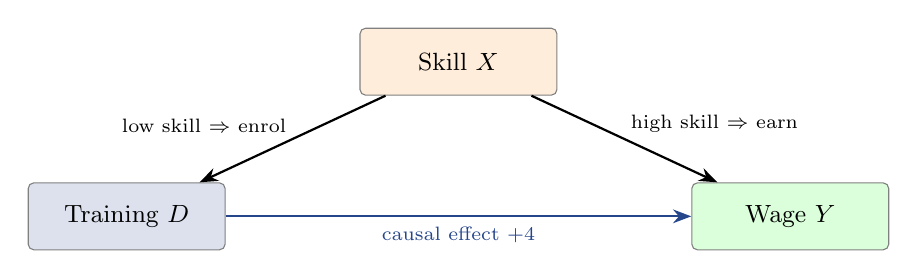
\begin{tikzpicture}[font=\small,>=Stealth,
      node distance=1.1cm and 2.6cm,
      var/.style={draw=black!50,rounded corners=2pt,minimum width=2.5cm,minimum height=0.85cm,align=center}]
    \node[var,fill=orange!14] (S) {Skill $X$};
    \node[var,fill=accent!16,below left=1.1cm and 1.7cm of S] (D) {Training $D$};
    \node[var,fill=green!14,below right=1.1cm and 1.7cm of S] (Y) {Wage $Y$};
    \draw[->,thick] (S) -- (D) node[midway,above left=-2pt]{\scriptsize low skill $\Rightarrow$ enrol};
    \draw[->,thick] (S) -- (Y) node[midway,above right=-2pt]{\scriptsize high skill $\Rightarrow$ earn};
    \draw[->,thick,accent] (D) -- (Y) node[midway,below]{\scriptsize causal effect $+4$};
  \end{tikzpicture}
  \end{center}
  \begin{readme}[Reading the diagram]
    The naive comparison measures \emph{both} arrows into $Y$: the causal path
    $D\to Y$ \textbf{plus} the backdoor path $D \leftarrow X \to Y$. Comparing within
    skill strata closes the backdoor --- but only for confounders you \emph{observe};
    motivation, health or ability would confound invisibly.
  \end{readme}
  \begin{industry}[Marketing: attribution]
    ``Customers who saw the ad bought $30\%$ more'' --- but the ad was targeted at likely
    buyers. Until a randomised holdout (ghost ads) says otherwise, that lift is
    selection, not persuasion.
  \end{industry}
\end{frame}

% ============================================================
\section{Potential Outcomes}
% ============================================================

\begin{frame}{The Neyman--Rubin framework: two outcomes per unit, one observed}
  \begin{block}{Potential outcomes and estimands}
    Each unit $i$ carries \emph{two} potential outcomes: $Y_i(1)$ if treated, $Y_i(0)$
    if not; the individual effect is $\tau_i = Y_i(1)-Y_i(0)$. We observe only
    \[
      \boxed{\;Y_i \;=\; D_i\,Y_i(1) + (1-D_i)\,Y_i(0).\;}
    \]
    Estimands: \ $\text{ATE}=E[\tau_i]$, \quad $\text{ATT}=E[\tau_i\mid D_i=1]$, \quad
    $\text{ATU}=E[\tau_i\mid D_i=0]$, with $\text{ATE}=\pi\,\text{ATT}+(1-\pi)\,\text{ATU}$.
  \end{block}
  \begin{readme}
    \begin{itemize}
      \item $Y_i(1),Y_i(0)$ exist \emph{before} treatment is decided --- treatment only
            selects which one you get to see.
      \item ATE: effect of treating \emph{everyone}; ATT: effect on those who were
            treated --- a mandatory rollout needs the ATE, a voluntary programme the ATT.
    \end{itemize}
  \end{readme}
  \begin{takeaway}[The fundamental problem of causal inference]
    No unit ever reveals both potential outcomes, so no $\tau_i$ is ever observed ---
    causal inference is a \textbf{missing-data problem}, with exactly half the data
    missing by construction.
  \end{takeaway}
\end{frame}

\begin{frame}{The God's-eye view: a potential-outcomes table}
  \begin{center}
    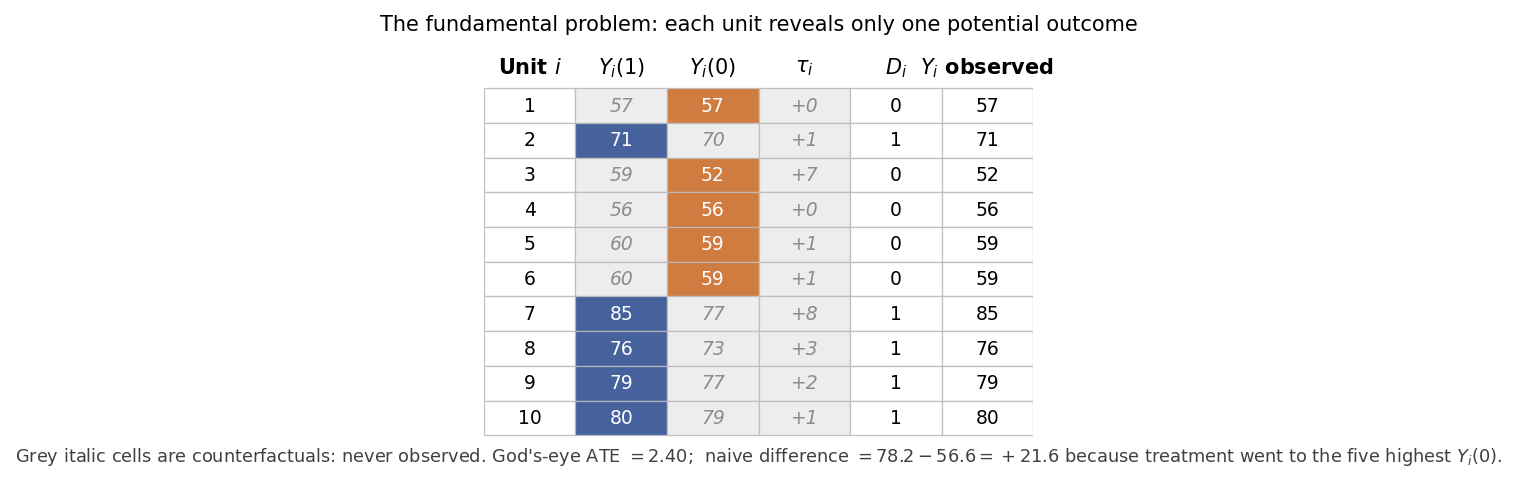
\includegraphics[width=0.88\textwidth,height=0.60\textheight,keepaspectratio]{cha1_po_table.png}
  \end{center}
  \begin{takeaway}
    In this simulated table the true ATE is $\mathbf{+2.40}$ (and ATT $=3.00$, ATU $=1.80$).
    An analyst sees only the coloured cells; because treatment went to the five highest
    $Y_i(0)$, the naive difference is $78.2-56.6=\mathbf{+21.6}$ --- nine times the truth.
  \end{takeaway}
\end{frame}

\begin{frame}{SUTVA --- the assumption the whole notation rests on}
  \begin{block}{Stable Unit Treatment Value Assumption}
    Writing $Y_i(1),Y_i(0)$ at all assumes: \ (i) \textbf{no interference} --- unit $i$'s
    outcome does not depend on \emph{other} units' treatments; \ (ii) \textbf{one version
    of treatment} --- ``treated'' means the same thing for every unit.
  \end{block}
  \begin{readme}[Where it honestly fails]
    \begin{itemize}
      \item Vaccination trials: my risk falls when \emph{you} are vaccinated (herd immunity).
      \item Marketplace tests: a discount for treated buyers depletes inventory or driver
            supply for the controls --- the control group is contaminated.
      \item Social features: ``invite your friends'' spills across arms by design.
    \end{itemize}
    SUTVA is a claim about the \emph{world}, not a modelling choice --- and randomisation
    does \textbf{not} buy it. When it fails, redefine the unit (clusters, regions,
    time slices) so that it holds.
  \end{readme}
  \begin{industry}[Two-sided marketplaces]
    Ride-hailing platforms test rider discounts with \emph{switchback} designs ---
    whole city--hour blocks are treated or not --- precisely because rider-level
    randomisation violates no-interference through the shared driver pool.
  \end{industry}
\end{frame}

\begin{frame}{Why the naive comparison lies: the selection-bias decomposition}
  \begin{block}{Derivation (two lines)}
    \vspace{-6pt}
    \begin{align*}
      E[Y\mid D=1]-E[Y\mid D=0]
        &= E[Y(1)\mid D=1]-E[Y(0)\mid D=0] \\
        &= \underbrace{E[Y(1)-Y(0)\mid D=1]}_{\text{ATT}}
           + \underbrace{E[Y(0)\mid D=1]-E[Y(0)\mid D=0]}_{\text{selection bias}}
    \end{align*}
    \vspace{-8pt}
    \[
      \boxed{\;\text{naive difference} \;=\; \text{ATT} \;+\; \text{selection bias}.\;}
    \]
  \end{block}
  \begin{readme}
    First line: each group reveals its own potential outcome. Second line: add and
    subtract $E[Y(0)\mid D=1]$ --- the \emph{counterfactual} of the treated. Selection
    bias asks: how would the treated have differed \textbf{anyway}, untreated?
    (Replacing ATT by ATE adds a third term, $(1-\pi)(\text{ATT}-\text{ATU})$ ---
    Exercise A1.2.)
  \end{readme}
  \begin{numexample}[The training programme decomposed]
    $-8.07 = \underbrace{3.97}_{\text{ATT}} + \underbrace{(-12.04)}_{\text{selection bias}}$:
    the trained (mostly low-skill) would have earned \$$12\,000$ \emph{less} even without
    training --- selection bias three times the size of the effect, with the opposite sign.
  \end{numexample}
\end{frame}

% ------------------------------------------------------------
\begin{frame}{Exercise A1.1 --- Potential outcomes by hand [Concept]}
\begin{exercise}
  Six workers have the following (God's-eye) potential outcomes; $D_i$ marks who actually
  took the training:
  \[
    \begin{array}{c|cccccc}
      i      & 1 & 2 & 3 & 4  & 5 & 6 \\ \hline
      Y_i(1) & 5 & 9 & 6 & 11 & 6 & 11 \\
      Y_i(0) & 4 & 7 & 3 & 9  & 5 & 8 \\
      D_i    & 0 & 1 & 0 & 1  & 0 & 1
    \end{array}
  \]
  \begin{enumerate}
    \item Compute every individual effect $\tau_i$ and the ATE.
    \item Which outcomes does the analyst actually observe? Is any $\tau_i$ observable?
    \item Compute the naive difference in observed means.
    \item Explain the gap using the decomposition: compute ATT and the selection-bias term.
  \end{enumerate}
\end{exercise}
\end{frame}

\begin{frame}{Solution --- Exercise A1.1}
\begin{solutionbox}
  \textbf{Part 1 --- effects.} $\tau = (1,2,3,2,1,3)$, so
  $\text{ATE} = \tfrac{1+2+3+2+1+3}{6} = \mathbf{2.0}$.

  \smallskip
  \textbf{Part 2 --- observed data.} Only $Y_2(1)=9$, $Y_4(1)=11$, $Y_6(1)=11$ and
  $Y_1(0)=4$, $Y_3(0)=3$, $Y_5(0)=5$. No unit shows both potential outcomes, so no
  $\tau_i$ is observable --- the fundamental problem.

  \smallskip
  \textbf{Part 3 --- naive difference.}
  $\bar Y_1 - \bar Y_0 = \tfrac{9+11+11}{3} - \tfrac{4+3+5}{3} = 10.33 - 4.00 = \mathbf{6.33}$
  --- more than three times the ATE.

  \smallskip
  \textbf{Part 4 --- decomposition.}
  $\text{ATT} = \tfrac{2+2+3}{3} = 2.33$; \ selection bias
  $= E[Y(0)\mid D{=}1] - E[Y(0)\mid D{=}0] = \tfrac{7+9+8}{3} - 4 = 8 - 4 = 4.00$.
  Check: $2.33 + 4.00 = 6.33$ \checkmark. Treatment went to workers who would have done
  better anyway.
\end{solutionbox}
\begin{mistake}
  Calling $\text{naive} - \text{ATE} = 4.33$ ``the'' selection bias. The exact bias term is
  $E[Y(0)\mid D{=}1]-E[Y(0)\mid D{=}0]=4.00$; the remaining $0.33$ is the ATT--ATE gap
  (treatment effects differ across groups).
\end{mistake}
\end{frame}

\begin{frame}{Exercise A1.2 --- The three-term decomposition [Math]}
\begin{exercise}
  Let $\pi = \Pr(D=1)$. Starting from
  $\;\text{naive} = \text{ATT} + \text{selection bias}\;$ and the identity
  $\text{ATE} = \pi\,\text{ATT} + (1-\pi)\,\text{ATU}$:
  \begin{enumerate}
    \item Show that
          $\;\text{naive} = \text{ATE} + \text{selection bias} +
          (1-\pi)\,(\text{ATT}-\text{ATU})$.
    \item Interpret the third term in one sentence.
    \item Verify the formula on the table of Exercise A1.1 (there $\pi = \tfrac12$).
  \end{enumerate}
\end{exercise}
\end{frame}

\begin{frame}{Solution --- Exercise A1.2}
\begin{solutionbox}
  \textbf{Part 1 --- derivation.} From the identity,
  \[
    \text{ATT}-\text{ATE} = \text{ATT} - \pi\,\text{ATT} - (1-\pi)\,\text{ATU}
    = (1-\pi)\,(\text{ATT}-\text{ATU}).
  \]
  Substituting $\text{ATT} = \text{ATE} + (1-\pi)(\text{ATT}-\text{ATU})$ into the
  two-term decomposition gives
  \[
    \text{naive} = \text{ATE} + \underbrace{E[Y(0)\mid D{=}1]-E[Y(0)\mid D{=}0]}_{\text{selection bias}}
    + \underbrace{(1-\pi)(\text{ATT}-\text{ATU})}_{\text{differential effect}} .
  \]
  \textbf{Part 2 --- interpretation.} Even with no baseline selection, the naive
  difference misses the ATE when those who take treatment \emph{benefit differently}
  from those who do not.

  \smallskip
  \textbf{Part 3 --- check.} $\text{ATU} = \tfrac{1+3+1}{3} = 1.67$, so
  $2.00 + 4.00 + \tfrac12(2.33-1.67) = 2.00 + 4.00 + 0.33 = 6.33$ \checkmark\ ---
  exactly the naive difference of A1.1. (In the training programme:
  $-8.07 = 4.07 - 12.04 - 0.10$.)
\end{solutionbox}
\begin{mistake}
  Believing ``no selection bias'' makes the naive comparison equal the ATE. It equals the
  \emph{ATT}; the differential-effect term must also vanish before it equals the ATE.
\end{mistake}
\end{frame}

% ============================================================
\section{Randomisation}
% ============================================================

\begin{frame}{Randomisation kills both bias terms --- in expectation}
  \begin{block}{What a coin flip buys}
    Random assignment forces $D \perp (Y(1),Y(0))$, hence
    $E[Y(0)\mid D{=}1] = E[Y(0)\mid D{=}0]$ (selection bias $=0$) and
    $\text{ATT}=\text{ATU}=\text{ATE}$. The naive comparison becomes the estimand:
    \[
      \boxed{\;E[Y\mid D=1]-E[Y\mid D=0] \;=\; \tau.\;}
    \]
  \end{block}
  \begin{readme}
    The coin cannot peek at $Y_i(0)$ or $Y_i(1)$ --- treated and control are random
    samples of the \emph{same} population, so \textbf{all} confounders, observed and
    unobserved, balance in expectation. That last clause is the entire magic: no list of
    control variables is ever needed, or ever complete.
  \end{readme}
  \begin{takeaway}
    ``In expectation'' is doing real work: any \emph{single} randomisation can be
    unlucky. The standard error on the next slide quantifies exactly that design noise
    --- bias is gone, variance remains.
  \end{takeaway}
  \begin{industry}[A/B testing is the RCT of tech]
    Hashing a user id into variant A or B \emph{is} the coin flip. The multi-billion
    experimentation industry --- feature flags, holdouts, ramp-ups --- is this one
    identity, run at the scale of $10^4$ experiments a year per platform.
  \end{industry}
\end{frame}

\begin{frame}{The difference in means, its standard error --- and Ch.\ 0}
  \begin{block}{Estimator, standard error, test}
    \[
      \hat\tau = \bar Y_1 - \bar Y_0, \qquad
      \widehat{\mathrm{SE}} = \sqrt{\frac{S_1^2}{n_1} + \frac{S_0^2}{n_0}}, \qquad
      \hat\tau \pm z_{0.975}\,\widehat{\mathrm{SE}}, \qquad
      t = \frac{\hat\tau}{\widehat{\mathrm{SE}}}.
    \]
  \end{block}
  \begin{readme}[This is the pre-course two-sample $t$-test]
    Identical to the Welch statistic from the Chapter~0 refresher: the humble $t$-test
    \emph{is} a complete RCT analysis. Neyman (1923) showed this SE is (weakly)
    \textbf{conservative} for the randomisation variance --- the honest direction to err
    (derivation in the appendix).
  \end{readme}
  \begin{numexample}[Training population --- randomised for once]
    Assign $500/500$ at random: one draw gives $\widehat{\mathrm{SE}} \approx 0.70$.
    Across $2000$ re-randomisations, the estimator's actual standard deviation is
    $0.70$ --- the formula tracks the true design variability.
  \end{numexample}
\end{frame}

\begin{frame}{Seeing it: the estimator's sampling distribution under both designs}
  \begin{center}
    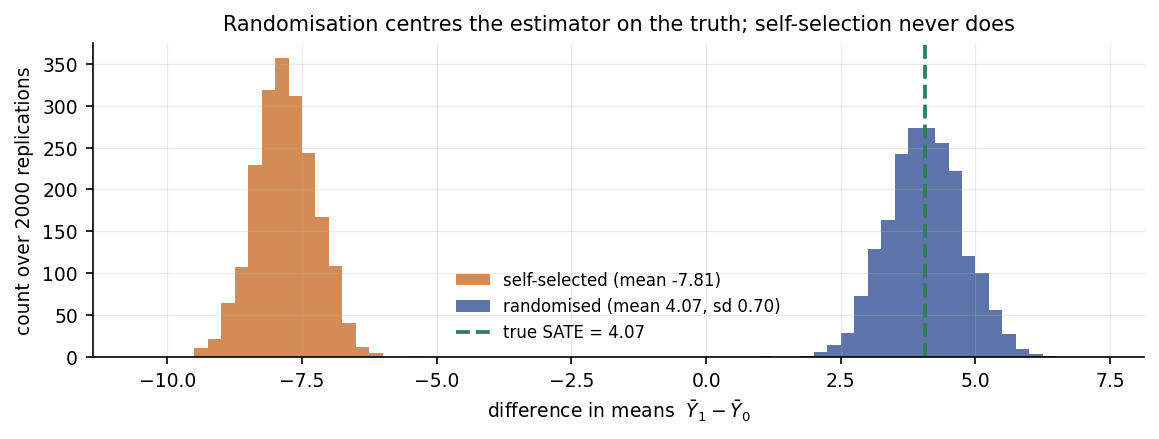
\includegraphics[width=0.90\textwidth,height=0.56\textheight,keepaspectratio]{cha1_sampling.png}
  \end{center}
  \begin{takeaway}
    Same population, $2000$ replications. Randomised (blue): mean $4.07$ --- exactly the
    truth $4.07$ --- sd $0.70$, and the $95\%$ CI covers the truth in $\mathbf{95.1\%}$ of
    draws. Self-selected (orange): mean $-7.81$, a structural bias of $-11.9$ that
    \textbf{no sample size reduces} --- the orange histogram is narrow \emph{and} wrong.
  \end{takeaway}
\end{frame}

% ------------------------------------------------------------
\begin{frame}{Exercise A1.3 --- Analysing a small RCT [Math]}
\begin{exercise}
  A randomised experiment ends with $n_1 = n_0 = 100$, treated mean
  $\bar Y_1 = 54.0$ ($S_1 = 10$), control mean $\bar Y_0 = 50.0$ ($S_0 = 10$).
  \begin{enumerate}
    \item Compute $\hat\tau$ and its standard error.
    \item Compute the $t$-statistic and the $95\%$ confidence interval
          (use $t_{0.975,\,198} = 1.972$).
    \item Decide at $\alpha = 0.05$ and state the conclusion in one honest sentence.
    \item What happens to the SE if both arms are doubled to $200$?
  \end{enumerate}
\end{exercise}
\end{frame}

\begin{frame}{Solution --- Exercise A1.3}
\begin{solutionbox}
  \textbf{Part 1.} $\hat\tau = 54.0 - 50.0 = 4.0$;
  $\widehat{\mathrm{SE}} = \sqrt{\tfrac{100}{100} + \tfrac{100}{100}} = \sqrt2 = 1.414$.

  \smallskip
  \textbf{Part 2.} $t = 4.0/1.414 = 2.83$; \ CI:
  $4.0 \pm 1.972 \times 1.414 = [\,1.21,\; 6.79\,]$; \ $p \approx 0.005$.

  \smallskip
  \textbf{Part 3.} Reject $H_0\!: \tau = 0$. ``Treatment raised the outcome by an
  estimated $4.0$ points ($95\%$ CI $1.2$ to $6.8$)'' --- because assignment was
  randomised, this difference \emph{is} the causal effect estimate, not a correlation.

  \smallskip
  \textbf{Part 4.} $\widehat{\mathrm{SE}} = \sqrt{\tfrac{100}{200}+\tfrac{100}{200}} = 1.0$:
  doubling both arms shrinks the SE by $1/\sqrt2$ --- precision is bought at quadratic
  cost, which is why power planning (Section 5) comes \emph{before} launch.
\end{solutionbox}
\begin{mistake}
  Computing the SE as if the $200$ observations were one sample
  ($S/\sqrt{200} = 0.71$). The SE of a \emph{difference} adds the two arms' variances ---
  it is $\sqrt2$ times larger.
\end{mistake}
\end{frame}

\begin{frame}{Extended Exercise A1.1 --- Randomisation vs selection in simulation [Python]}
\begin{longexercise}
  Build the training population from the lecture with \texttt{np.random.default\_rng(2024)}:
  \texttt{high} $\sim$ Bernoulli($0.5$), enrolment probability $0.8/0.2$ for low/high skill,
  $Y(0) = 40 + 20\,\texttt{high} + \mathcal N(0,5^2)$,
  $\tau = 4 + \mathcal N(0,2^2)$, $Y(1)=Y(0)+\tau$, $n=1000$.
  \begin{enumerate}
    \item Simulate $2000$ replications of (a) \textbf{self-selected} uptake and
          (b) \textbf{randomised} $500/500$ assignment; record the difference in means.
    \item Report mean and sd of both estimator distributions, and the bias of (a).
    \item Under randomisation, compute the coverage of the $95\%$ CI
          $\hat\tau \pm 1.96\,\widehat{\mathrm{SE}}$.
    \item In two sentences: what does randomisation fix, and what does it not fix?
  \end{enumerate}
\end{longexercise}
\begin{labnote}[Run this live]
  The worked solution sits in \texttt{advanced\_01\_rcts\_lab.ipynb} under
  \emph{Lecture exercises --- worked Python solutions}: the cell headed
  \emph{Extended Exercise A1.1 --- Randomisation vs selection in simulation [Python]}.
\end{labnote}
\end{frame}

\begin{frame}[fragile]{Solution --- Extended Exercise A1.1 (1/2)}
\begin{solutionbox}[Solution --- code: population and the two designs]
\begin{lstlisting}[basicstyle=\ttfamily\scriptsize]
import numpy as np
rng = np.random.default_rng(2024)                    # module seed
n = 1000
high = rng.random(n) < 0.5                           # skill stratum
p_sel = np.where(high, 0.2, 0.8)                     # self-selection propensities
_ = rng.random(n) < p_sel                            # the observational draw
y0 = 40 + 20*high + rng.normal(0, 5, n)              # potential outcome untreated
tau = 4 + rng.normal(0, 2, n)                        # heterogeneous ITEs, mean 4
y1 = y0 + tau                                        # potential outcome treated

est_r, est_s, cover = [], [], 0
for _ in range(2000):                                # 2000 replications
    Dr = np.zeros(n, bool); Dr[rng.permutation(n)[:500]] = True   # randomised
    yr = np.where(Dr, y1, y0)
    d = yr[Dr].mean() - yr[~Dr].mean(); est_r.append(d)
    se = np.sqrt(yr[Dr].var(ddof=1)/500 + yr[~Dr].var(ddof=1)/500)
    cover += abs(d - tau.mean()) <= 1.96*se          # CI covers truth?
    Ds = rng.random(n) < p_sel                       # self-selected uptake
    ys = np.where(Ds, y1, y0)
    est_s.append(ys[Ds].mean() - ys[~Ds].mean())
\end{lstlisting}
\end{solutionbox}
\end{frame}

\begin{frame}{Solution --- Extended Exercise A1.1 (2/2)}
\begin{solutionbox}[Solution --- numbers and interpretation]
  \textbf{Parts 2--3 --- printout} (true SATE $= 4.07$):
  \begin{center}\ttfamily\footnotesize
  randomised\quad mean 4.07\quad sd 0.70\quad coverage 0.951\\[2pt]
  self-selected\quad mean -7.81\quad sd 0.56\quad bias -11.88
  \end{center}
  \begin{itemize}
    \item \textbf{Randomised}: centred on the truth; the Neyman CI covers it in
          $95.1\%$ of draws --- the advertised guarantee, delivered.
    \item \textbf{Self-selected}: bias $-11.9$, stable across replications ---
          collecting the same biased data $2000$ times over changes nothing.
  \end{itemize}
  \textbf{Part 4.} Randomisation removes \emph{bias} (both decomposition terms are zero
  in expectation); it does not remove \emph{variance} --- a single unlucky draw can still
  be off, which is what the SE and CI quantify. It also does not buy SUTVA or fix
  attrition and non-compliance (Section 6).
\end{solutionbox}
\begin{mistake}
  Expecting the self-selected estimator to be \emph{noisier}. It is actually slightly
  \emph{more} stable here (sd $0.56$ vs $0.70$) --- precision is no defence against bias;
  a tight interval around the wrong number is the most dangerous output in statistics.
\end{mistake}
\end{frame}

% ============================================================
\section{Regression Adjustment}
% ============================================================

\begin{frame}{Should we adjust an RCT with regression? (bridge to Ch.\ 3)}
  \begin{block}{Regression adjustment}
    Fit the Chapter~3 model on experimental data:
    \[
      Y_i = \alpha + \tau D_i + X_i^\top\beta + \varepsilon_i .
    \]
    Randomisation makes $X \perp D$, so $\hat\tau$ still estimates the ATE --- the
    covariates soak up outcome variance and \textbf{shrink the standard error}.
  \end{block}
  \begin{readme}[The rules that keep it honest]
    \begin{itemize}
      \item Covariates must be \textbf{pre-treatment} (measured before assignment) and
            \textbf{pre-specified} (chosen before results are seen).
      \item Adjustment here buys \emph{precision}, not identification --- unlike in
            observational data, the estimate is valid even with \emph{no} covariates.
      \item With very unequal arms or strong effect heterogeneity, add
            $D\times(X-\bar X)$ interactions (Lin 2013) --- the safe default at scale.
    \end{itemize}
  \end{readme}
  \begin{mistake}
    Trying covariate sets until $\hat\tau$ is significant. That is $p$-hacking with extra
    steps --- Chapter~13 in new clothes. One pre-registered specification, reported
    whatever it says.
  \end{mistake}
\end{frame}

\begin{frame}[fragile]{A semi-synthetic experiment on Wage ($n=3000$)}
  Real covariates and wages from \texttt{Wage.csv}; we \emph{randomise} a fake programme
  and build in a true effect of $+5$:
  \begin{lstlisting}
import numpy as np, pandas as pd
import statsmodels.formula.api as smf
wage = pd.read_csv("Wage.csv")                    # course data, n = 3000
rng = np.random.default_rng(2024)
wage["D"] = (rng.random(len(wage)) < 0.5).astype(int)  # coin flip: 1475 vs 1525
wage["y"] = wage["wage"] + 5.0 * wage["D"]        # truth by construction: tau = 5

m0 = smf.ols("y ~ D", data=wage).fit(cov_type="HC2")   # robust (HC2) SEs
print(m0.params["D"], m0.bse["D"])                # 4.122  1.523
  \end{lstlisting}
  \begin{readme}[Why \texttt{cov\_type="HC2"}]
    Treatment may change the \emph{variance} of $Y$, not just its mean; classical OLS
    SEs assume equal error variance across arms. Heteroskedasticity-consistent (HC)
    errors drop that assumption --- HC2 exactly reproduces the Neyman variance in a
    two-arm experiment, so it is the natural default for RCTs.
  \end{readme}
\end{frame}

\begin{frame}{What adjustment buys: the numbers}
  \begin{numexample}[Unadjusted vs adjusted --- true effect $+5$; HC2 SEs]
    \begin{center}\footnotesize
    \begin{tabular}{@{}lccc@{}}
      \toprule
      Model & $\hat\tau$ & SE & $95\%$ CI \\
      \midrule
      \texttt{y \~{} D}                     & $4.12$ & $1.52$ & $[1.14,\ 7.11]$ \\
      \texttt{y \~{} D + age + education}   & $3.73$ & $1.31$ & $[1.15,\ 6.31]$ \\
      \bottomrule
    \end{tabular}
    \end{center}
    SE ratio $0.86$ $\Rightarrow$ variance down $25\%$ $\Rightarrow$ worth $34\%$ more
    sample, for free. The covariates explain $R^2 \approx 0.26$ of the outcome ---
    that is the fuel of the precision gain.
  \end{numexample}
  \begin{takeaway}
    Adjustment buys \textbf{precision, not truth}: both estimates are unbiased and both
    CIs cover the built-in $+5$; the adjusted one is simply less noisy. The estimates
    differ ($4.12$ vs $3.73$) only through sampling noise --- with one finite
    randomisation, that is expected, not alarming.
  \end{takeaway}
  \begin{industry}[CUPED: the same idea at scale]
    Tech platforms adjust for the \emph{same metric measured pre-experiment}
    (CUPED). Variance reductions around $50\%$ are routine --- halving every
    experiment's duration is worth more than any modelling refinement.
  \end{industry}
\end{frame}

% ------------------------------------------------------------
\begin{frame}{Exercise A1.4 --- Regression adjustment on the Wage experiment [Python]}
\begin{exercise}
  Using \texttt{Wage.csv} and the semi-synthetic experiment from the lecture
  (seed $2024$, coin-flip $D$, $y = \texttt{wage} + 5D$):
  \begin{enumerate}
    \item Fit the unadjusted model \texttt{y \~{} D} with HC2 standard errors and report
          $\hat\tau$ and its SE.
    \item Add \texttt{age} and \texttt{education}; report the new $\hat\tau$ and SE.
    \item Compute the implied variance reduction and the equivalent sample-size gain.
    \item A colleague proposes also adjusting for a satisfaction survey answered
          \emph{after} the programme. Why must you refuse?
  \end{enumerate}
\end{exercise}
\begin{labnote}[Run this live]
  The worked solution sits in \texttt{advanced\_01\_rcts\_lab.ipynb} under
  \emph{Lecture exercises --- worked Python solutions}: the cell headed
  \emph{Exercise A1.4 --- Regression adjustment on the Wage experiment [Python]}.
\end{labnote}
\end{frame}

\begin{frame}[fragile]{Solution --- Exercise A1.4 (1/2)}
\begin{solutionbox}[Solution --- code]
\begin{lstlisting}
import numpy as np, pandas as pd
import statsmodels.formula.api as smf
wage = pd.read_csv("Wage.csv")                     # n = 3000
rng = np.random.default_rng(2024)                  # lecture seed
wage["D"] = (rng.random(len(wage)) < 0.5).astype(int)
wage["y"] = wage["wage"] + 5.0 * wage["D"]         # true effect +5

m0 = smf.ols("y ~ D", data=wage).fit(cov_type="HC2")
m1 = smf.ols("y ~ D + age + education", data=wage).fit(cov_type="HC2")
print(round(m0.params["D"], 3), round(m0.bse["D"], 3))   # 4.122 1.523
print(round(m1.params["D"], 3), round(m1.bse["D"], 3))   # 3.732 1.315
\end{lstlisting}
\end{solutionbox}
\end{frame}

\begin{frame}{Solution --- Exercise A1.4 (2/2)}
\begin{solutionbox}[Solution --- reading the output]
  \textbf{Parts 1--2.} Unadjusted: $\hat\tau = 4.122$ (SE $1.523$). Adjusted:
  $\hat\tau = 3.732$ (SE $1.315$). Both within one SE of the built-in truth $+5$.

  \smallskip
  \textbf{Part 3.} Variance ratio $(1.315/1.523)^2 = 0.746$: adjustment cut the variance
  by $25.4\%$. Equivalent sample gain: $1/0.746 = 1.34$ --- the adjusted analysis of
  $3000$ people is as precise as an unadjusted one of about $4000$.

  \smallskip
  \textbf{Part 4.} The survey is \textbf{post-treatment}: the programme may change
  satisfaction, so conditioning on it splits the sample by a \emph{consequence} of $D$
  --- a ``bad control'' that re-introduces exactly the selection bias randomisation
  eliminated. Only pre-treatment covariates are admissible.
\end{solutionbox}
\begin{mistake}
  Reading $\hat\tau$ moving from $4.12$ to $3.73$ as the adjusted model ``finding a
  smaller effect''. Both estimate the same $\tau$; the wobble is sampling noise. What
  changed systematically is the \emph{SE} --- that is the whole point of adjusting.
\end{mistake}
\end{frame}

% ============================================================
\section{Design \& Power}
% ============================================================

\begin{frame}{Power and the minimum detectable effect}
  \begin{block}{Sample size for a two-arm trial (equal arms, two-sided $\alpha$)}
    \[
      \boxed{\;n_{\text{per arm}} \;=\; \frac{2\,\sigma^2\,(z_{1-\alpha/2}+z_{1-\beta})^2}{\delta^2}\;}
      \qquad\Longleftrightarrow\qquad
      \mathrm{MDE} = (z_{1-\alpha/2}+z_{1-\beta})\;\sigma\,\sqrt{\tfrac{2}{n}} .
    \]
  \end{block}
  \begin{readme}
    \begin{itemize}
      \item $\sigma$: outcome sd; \ $\delta$: smallest effect worth detecting; \
            $\alpha$: test size; \ $1-\beta$: power.
      \item For $\alpha=0.05$, power $80\%$: $z_{0.975}=1.96$, $z_{0.80}=0.84$, so
            $(z_{1-\alpha/2}+z_{1-\beta})^2 = 7.85$ --- the handy rule
            $n \approx 15.7\,\sigma^2/\delta^2$ per arm.
      \item The MDE is the same equation read backwards: given my $n$, what can I
            honestly hope to see?
    \end{itemize}
  \end{readme}
  \begin{numexample}[The wage experiment --- planned properly]
    $\sigma = 41.7$ (sd of \texttt{wage}), $\delta = 5$:
    $n = 2 \times 7.85 \times 41.7^2 / 25 = \mathbf{1094}$ per arm. Conversely, at
    $n=1000$ per arm the MDE is $2.80 \times 41.7 \times \sqrt{2/1000} = \mathbf{5.23}$.
  \end{numexample}
\end{frame}

\begin{frame}{The power curve: analytic formula vs simulation (bridge to Ch.\ 5)}
  \begin{center}
    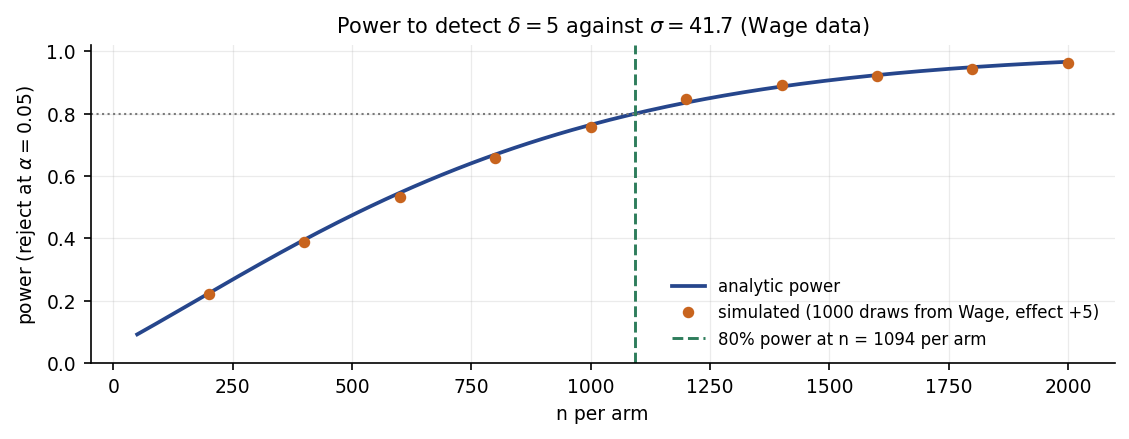
\includegraphics[width=0.88\textwidth,height=0.56\textheight,keepaspectratio]{cha1_power.png}
  \end{center}
  \begin{takeaway}
    Orange dots: $1000$ simulated experiments per $n$, resampling real \texttt{Wage} data
    with a $+5$ effect --- at $n=500$ the simulation says $0.477$, the formula $0.474$.
    Both agree: $80\%$ power needs $\mathbf{1094}$ per arm; at $500$ per arm you toss a
    slightly bent coin.
  \end{takeaway}
  \begin{mistake}
    Running underpowered and reading ``not significant'' as ``no effect''. At $47\%$
    power, a real $+5$ effect is \emph{missed} more often than found --- absence of
    evidence, not evidence of absence.
  \end{mistake}
\end{frame}

\begin{frame}{Design refinements: blocking and cluster randomisation}
  \begin{block}{Stratified (blocked) randomisation}
    Randomise \emph{within} strata of a prognostic variable (skill, country, device).
    Balance on the stratum is exact by construction, not just in expectation; analyse
    with stratum fixed effects. Precision gain $\approx$ regression adjustment,
    guaranteed by design.
  \end{block}
  \begin{block}{Cluster randomisation and the design effect}
    When treatment operates on groups (schools, cities, stores) or interference within
    groups breaks SUTVA, randomise \emph{clusters}. Outcomes within a cluster are
    correlated ($\rho$), so $n$ raw observations are worth fewer:
    \[
      \boxed{\;\mathrm{DE} = 1 + (m-1)\,\rho\;}
      \qquad n_{\text{effective}} = n / \mathrm{DE}.
    \]
  \end{block}
  \begin{numexample}
    $200$ schools $\times$ $50$ pupils, $\rho = 0.05$:
    $\mathrm{DE} = 1 + 49 \times 0.05 = \mathbf{3.45}$ --- the $10\,000$ pupils carry the
    information of $10\,000/3.45 \approx \mathbf{2899}$ independent ones.
  \end{numexample}
  \begin{industry}[Geo experiments]
    Brand and TV campaigns cannot randomise users, so platforms randomise \emph{regions}.
    Few, large, heterogeneous clusters make the design effect brutal --- which is why geo
    tests run for months while user-level A/B tests run for weeks.
  \end{industry}
\end{frame}

% ------------------------------------------------------------
\begin{frame}{Exercise A1.5 --- Sample size for an A/B test [Math]}
\begin{exercise}
  A sign-up funnel converts at $p_0 = 10\%$. You must detect an absolute lift of
  $2$ percentage points (to $p_1 = 12\%$) at $\alpha = 0.05$ (two-sided) with $80\%$
  power. For proportions, the per-arm sample size is
  \[
    n \;=\; \frac{(z_{1-\alpha/2}+z_{1-\beta})^2\,\big[p_0(1-p_0) + p_1(1-p_1)\big]}{(p_1-p_0)^2}.
  \]
  \begin{enumerate}
    \item Compute $n$ per arm (use $(z_{1-\alpha/2}+z_{1-\beta})^2 = 7.85$).
    \item The product owner halves the MDE to $1$ point ($p_1 = 11\%$). Recompute $n$.
    \item State the approximate scaling law of $n$ in the MDE $\delta$.
  \end{enumerate}
\end{exercise}
\end{frame}

\begin{frame}{Solution --- Exercise A1.5}
\begin{solutionbox}
  \textbf{Part 1.} Variance term: $0.10 \times 0.90 + 0.12 \times 0.88 = 0.1956$.
  \[
    n = \frac{7.85 \times 0.1956}{0.02^2} = \frac{1.535}{0.0004} \approx \mathbf{3839}
    \text{ per arm } (\approx 7700 \text{ users in total}).
  \]
  \textbf{Part 2.} Variance term: $0.10\times0.90 + 0.11\times0.89 = 0.1879$;
  \[
    n = \frac{7.85 \times 0.1879}{0.01^2} \approx \mathbf{14\,749} \text{ per arm}
    \quad (3.84\times \text{Part 1}).
  \]
  \textbf{Part 3.} $n \propto 1/\delta^2$: halving the detectable effect roughly
  \textbf{quadruples} the sample (here $3.84\times$, slightly less than $4$ because the
  variance term also shrinks as $p_1$ moves toward $p_0$). Sensitivity is the most
  expensive word in experimentation.
\end{solutionbox}
\begin{mistake}
  Quoting $n$ for a \emph{relative} lift as if it were absolute. A ``$2\%$ lift'' on a
  $10\%$ baseline is $0.2$ points, not $2$ --- a $100\times$ larger required sample.
  Always spell out absolute percentage points.
\end{mistake}
\end{frame}

% ============================================================
\section{Threats \& Practice}
% ============================================================

\begin{frame}{Attrition: the quiet return of selection bias}
  Randomisation happens at assignment --- but people \emph{leave} afterwards, and they do
  not leave at random.
  \begin{readme}[When dropout hurts --- and how to see it]
    \begin{itemize}
      \item Harmless: attrition unrelated to treatment and outcome (pure noise, less $n$).
      \item Harmful: \textbf{differential} attrition --- e.g.\ the control group's
            weakest participants quit, so the surviving controls look artificially strong.
      \item Diagnostics: compare attrition \emph{rates} by arm; compare
            \emph{pre-treatment covariates} of the stayers by arm; if suspicious, report
            worst-case (Manski/Lee) bounds rather than a point estimate.
    \end{itemize}
  \end{readme}
  \begin{takeaway}
    You randomised the \emph{assigned}; you analyse the \emph{observed}. The moment those
    two populations differ by arm, the selection-bias term of Section~2 is back --- with
    the same algebra and the same danger.
  \end{takeaway}
  \begin{mistake}
    Analysing ``completers only'' because the data are cleaner. That silently converts
    your RCT into an observational study of who persists.
  \end{mistake}
\end{frame}

\begin{frame}{Non-compliance and the intention-to-treat principle}
  People assigned to treatment ($Z_i = 1$) do not always take it ($D_i = 0$) --- and
  compliance is self-selected.
  \begin{block}{Intention-to-treat (ITT)}
    Compare by \emph{assignment}, ignoring uptake:
    \[
      \boxed{\;\widehat{\mathrm{ITT}} = \bar Y_{Z=1} - \bar Y_{Z=0}\;}
    \]
    $Z$ is randomised even when $D$ is not --- ITT inherits the full causal guarantee.
  \end{block}
  \begin{readme}
    ITT estimates the effect of \emph{offering} the treatment --- exactly the quantity a
    policy or product decision needs, since rollout can only ever offer. It is diluted
    by non-compliance: with compliance share $c$ and no effect on never-takers,
    $\mathrm{ITT} = c \times \text{effect on compliers}$.
  \end{readme}
  \begin{numexample}
    Compliance $75\%$, true effect on compliers $8$: the experiment shows
    $\mathrm{ITT} = 0.75 \times 8 = \mathbf{6.0}$ --- smaller, but honestly caused by the
    offer.
  \end{numexample}
\end{frame}

\begin{frame}{Per-protocol analysis vs the compliers' effect (CACE)}
  \begin{block}{Per-protocol: the tempting, biased alternative}
    Comparing those who \emph{took} treatment with everyone else discards
    randomisation: compliers are self-selected (keener, healthier, more engaged), so the
    selection-bias decomposition applies in full.
  \end{block}
  \begin{block}{The instrumental-variables repair}
    Under randomised $Z$, exclusion ($Z$ affects $Y$ only through $D$) and one-sided
    non-compliance:
    \[
      \boxed{\;\widehat{\mathrm{CACE}} = \frac{\widehat{\mathrm{ITT}}_Y}{\widehat{\mathrm{ITT}}_D}
      = \frac{\bar Y_{Z=1}-\bar Y_{Z=0}}{\text{compliance share}}\;}
    \]
    (the Wald estimator; derivation in the appendix).
  \end{block}
  \begin{numexample}
    $\widehat{\mathrm{CACE}} = 6.0 / 0.75 = \mathbf{8.0}$: the offer moved outcomes by
    $6.0$ on average \emph{because} the $75\%$ who complied gained $8.0$ each.
  \end{numexample}
  \begin{mistake}
    Dropping non-compliers ``to measure the real effect''. The real repair divides by the
    compliance share; it never deletes randomised units.
  \end{mistake}
\end{frame}


\begin{frame}{What non-compliance costs, drawn}
  \begin{center}
    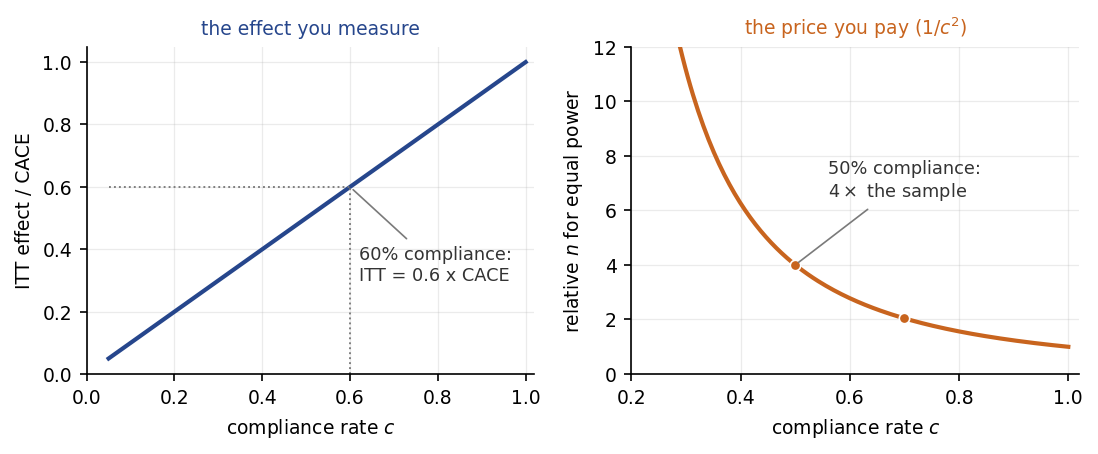
\includegraphics[width=0.90\textwidth,height=0.52\textheight,keepaspectratio]{cha1_itt_dilution.png}
  \end{center}
  \begin{takeaway}
    ITT is diluted \emph{linearly} by the compliance rate --- and because
    power depends on the effect squared, the sample size needed to detect the
    diluted effect grows as $1/c^2$: at $50\%$ compliance you need four
    times the participants. Compliance is a design problem, not an analysis
    problem.
  \end{takeaway}
\end{frame}

\begin{frame}{Balance checks: auditing the randomiser}
  \begin{center}
    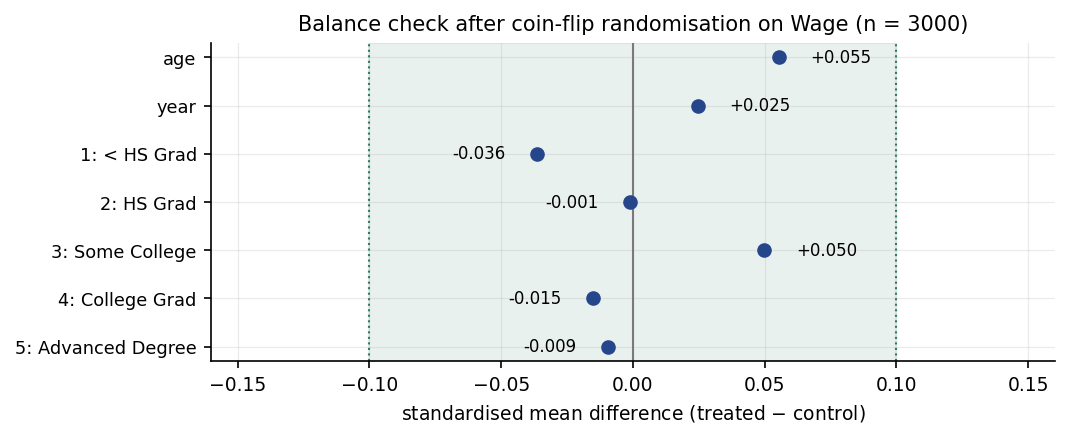
\includegraphics[width=0.86\textwidth,height=0.52\textheight,keepaspectratio]{cha1_balance.png}
  \end{center}
  \begin{takeaway}
    Standardised mean differences for the Wage experiment: every covariate sits within
    $\pm 0.06$ --- comfortably inside the $|\mathrm{SMD}| < 0.1$ rule of thumb (largest:
    age at $+0.055$). This is what a healthy randomisation looks like.
  \end{takeaway}
  \begin{mistake}[Balance-test theatre]
    Running $t$-tests on every covariate and panicking at one star: with a truly random
    $D$, $5\%$ of balance tests reject \emph{by construction} --- they audit your
    randomiser (bucketing bugs, broken hashing), not your design. Judge SMDs, and handle
    a chance imbalance on a prognostic covariate by (pre-specified) adjustment.
  \end{mistake}
\end{frame}

\begin{frame}{Peeking: multiple testing in the time dimension (bridge to Ch.\ 13)}
  \begin{center}
    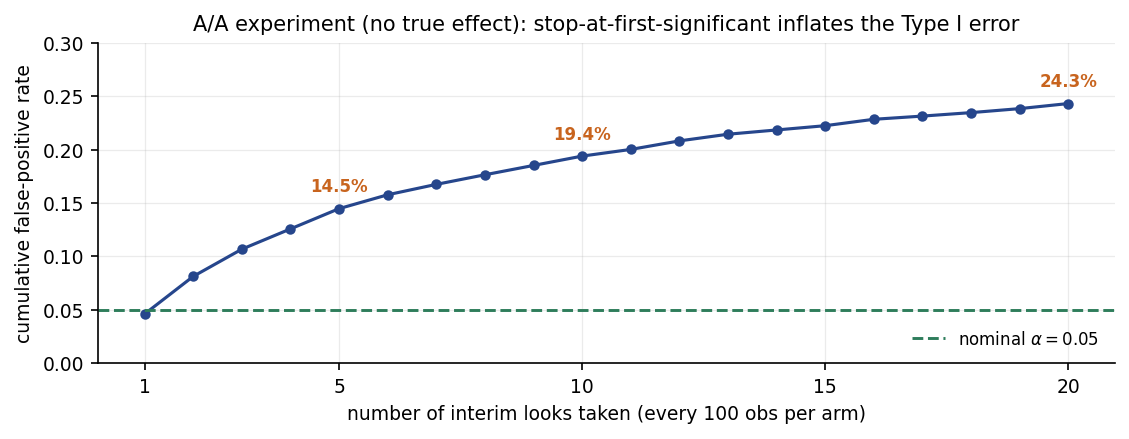
\includegraphics[width=0.86\textwidth,height=0.50\textheight,keepaspectratio]{cha1_peeking.png}
  \end{center}
  \begin{takeaway}
    An A/A test (no true effect), checked after every $100$ users per arm and stopped at
    the first star: the realised false-positive rate is $4.6\%$ after one look but
    $\mathbf{14.5\%}$ by $5$ looks, $\mathbf{19.4\%}$ by $10$, $\mathbf{24.3\%}$ by $20$.
    Each look is another test on overlapping data --- correlated, so below the
    independent-tests bound $1-0.95^{20}=64\%$, yet five times nominal $\alpha$.
  \end{takeaway}
  \begin{readme}[What to do instead]
    Fix the horizon in advance and look once; or pre-specify group-sequential boundaries
    (O'Brien--Fleming $\alpha$-spending); or use always-valid sequential inference.
    ``Significant when I looked'' is not an analysis plan.
  \end{readme}
  \begin{labnote}
    \S6 of \texttt{advanced\_01\_rcts\_lab.ipynb} reruns this simulation --- change the
    look frequency and watch the error rate move.
  \end{labnote}
\end{frame}

\begin{frame}{The A/B playbook: this module, spoken in tech}
  \scriptsize
  \begin{center}
  \begin{tabular}{@{}p{4.1cm}p{7.9cm}@{}}
    \toprule
    \textbf{This module} & \textbf{A/B practice} \\
    \midrule
    Unit and randomisation & User, assigned by hashing a stable id into variants \\
    Treatment $D$ & The variant behind a feature flag \\
    Primary outcome & One pre-registered north-star metric per experiment \\
    Power / MDE & Traffic forecast $\to$ MDE $\to$ run length, fixed in advance \\
    ITT & Analyse every \emph{bucketed} user, exposed or not \\
    SUTVA repair & Switchback / geo / cluster designs for marketplaces \\
    Peeking control & Fixed horizon, or sequential (always-valid) methods \\
    Secondary metrics, segments & FDR control and ``exploratory'' labels --- Chapter 13 \\
    \bottomrule
  \end{tabular}
  \end{center}
  \begin{industry}[A/B testing is the RCT of tech]
    Large platforms run tens of thousands of experiments a year; the experiment config
    \emph{is} the pre-registration, guardrail metrics are the safety endpoints, and the
    ramp-up plan is the dose escalation. Every hard problem in this section ---
    interference, peeking, multiplicity --- is a live engineering concern, not a
    textbook footnote.
  \end{industry}
\end{frame}

% ------------------------------------------------------------
\begin{frame}{Exercise A1.6 --- ITT, per-protocol and compliance [Concept]}
\begin{exercise}
  An app randomises $2000$ users $1{:}1$: the treatment arm is \emph{offered} a coaching
  feature; the control arm is not. In the offered arm, $75\%$ activate the feature;
  no control user can. The offered arm's mean engagement ends $6.0$ points above the
  control arm's.
  \begin{enumerate}
    \item State the ITT estimate. What causal quantity does it measure?
    \item An analyst proposes comparing the $750$ activators with all $1250$
          non-activating users (both arms pooled). What exactly is wrong?
    \item Estimate the effect on the users who actually activate (state your assumptions).
    \item Which number belongs in the rollout decision, and why?
  \end{enumerate}
\end{exercise}
\end{frame}

\begin{frame}{Solution --- Exercise A1.6}
\begin{solutionbox}
  \textbf{Part 1.} $\widehat{\mathrm{ITT}} = 6.0$ points: the causal effect of
  \emph{offering} the feature, guaranteed unbiased because the offer was randomised.

  \smallskip
  \textbf{Part 2.} Activators are self-selected --- the engaged users opt in. The
  comparison equals ATT $+$ selection bias (Section 2), and the bias term is almost
  surely positive here: activators would have been more engaged \emph{anyway}. It also
  pools controls with unmotivated treated users, muddying both sides.

  \smallskip
  \textbf{Part 3.} With one-sided non-compliance and exclusion ($Z$ moves engagement
  only via activation): $\widehat{\mathrm{CACE}} = 6.0/0.75 = \mathbf{8.0}$ points among
  compliers.

  \smallskip
  \textbf{Part 4.} The \textbf{ITT} ($6.0$): shipping the feature can only ever
  \emph{offer} it, so the offer effect is the rollout effect. The CACE ($8.0$) answers a
  different, product-design question --- how valuable the feature is to those who engage.
\end{solutionbox}
\begin{mistake}
  Reporting the CACE as ``the effect of the feature'' without the assumptions
  (randomised offer, exclusion, one-sidedness) --- and without saying it applies to
  compliers only, not to the average user.
\end{mistake}
\end{frame}

\begin{frame}{Extended Exercise A1.2 --- Designing the free-shipping experiment [Integrative]}
\begin{longexercise}
  An online shop converts $p_0 = 5.0\%$ of visitors. Marketing wants to test a
  free-shipping threshold and cares about an absolute lift of $0.5$ percentage points.
  Traffic: $20\,000$ visitors per week, split evenly between arms.
  \begin{enumerate}
    \item Compute the required sample per arm ($\alpha=0.05$, power $80\%$,
          $(z_{1-\alpha/2}+z_{1-\beta})^2=7.85$) and the run time in weeks.
    \item The product manager suggests checking daily and stopping at the first
          significant result. Quantify the danger and give two acceptable alternatives.
    \item Should you randomise \emph{sessions} or \emph{users}? Justify via SUTVA and
          independence.
    \item Twelve secondary metrics will be tracked. State a defensible reporting rule
          (bridge to Chapter 13).
  \end{enumerate}
\end{longexercise}
\end{frame}

\begin{frame}{Solution --- Extended Exercise A1.2 (1/2)}
\begin{solutionbox}[Solution --- power arithmetic and run time]
  \textbf{Part 1.} Variance term:
  $0.05\times0.95 + 0.055\times0.945 = 0.0475 + 0.0520 = 0.0995$.
  \[
    n = \frac{7.85 \times 0.0995}{0.005^2}
      = \frac{0.781}{0.000025} \approx \mathbf{31\,231} \text{ per arm}.
  \]
  At $10\,000$ visitors per arm per week: $31\,231/10\,000 \approx 3.1$ weeks
  $\Rightarrow$ \textbf{run 4 full weeks} --- rounding \emph{up} to whole weekly cycles
  keeps weekday/weekend mix balanced.

  \smallskip
  \textbf{MDE honesty check.} If management demanded an answer after one week
  ($10\,000$ per arm), the MDE would be
  $2.80\sqrt{2 \times 0.05 \times 0.95 / 10\,000} \approx 0.86$ points --- the test
  could \emph{not} see the $0.5$-point effect anyone cares about. Say so before launch,
  not after.
\end{solutionbox}
\end{frame}

\begin{frame}{Solution --- Extended Exercise A1.2 (2/2)}
\begin{solutionbox}[Solution --- peeking; units; metric discipline]
  \textbf{Part 2.} Daily checks over 4 weeks $=$ up to $28$ looks; the lecture's A/A
  simulation already reaches a $\mathbf{24.3\%}$ false-positive rate by $20$ looks ---
  roughly one ineffective change in four would ship. Alternatives: (i) fixed horizon,
  one look at 4 weeks; (ii) pre-specified group-sequential boundaries or always-valid
  sequential inference, which permit monitoring at controlled $\alpha$.

  \smallskip
  \textbf{Part 3.} Randomise \textbf{users}. Sessions of the same visitor are not
  independent, and a returning visitor would bounce between variants --- violating the
  ``one version of treatment'' half of SUTVA and contaminating both arms. (Analysing
  sessions while randomising users then requires cluster-robust SEs --- the design
  effect of Section 5.)

  \smallskip
  \textbf{Part 4.} Pre-register conversion as the \emph{primary} metric, judged at
  $\alpha=0.05$. Report the twelve secondaries with Benjamini--Hochberg FDR control and
  label anything found only in segments as \emph{exploratory} --- Chapter 13's rules,
  applied verbatim.
\end{solutionbox}
\begin{mistake}
  Treating the $3.1$-week answer as ``we can stop Wednesday of week 4''. The horizon
  was chosen to protect $\alpha$ and power --- stopping on schedule is part of the
  test's validity, not bureaucracy.
\end{mistake}
\end{frame}

% ============================================================
\section{Python Lab}
% ============================================================

\begin{frame}{Python lab --- run it live in the notebook}
  \begin{labnote}[Companion notebook: \texttt{advanced\_01\_rcts\_lab.ipynb}]
    The code in this module is meant to be \textbf{run, not read}. Open the companion
    Jupyter notebook and work through it cell by cell:
    \begin{itemize}
      \item \S1, \emph{A confounded training programme} --- simulate the population;
            naive vs stratified comparisons;
      \item \S2, \emph{Potential outcomes and selection bias} --- the God's-eye view and
            the decomposition, term by term;
      \item \S3, \emph{Randomisation in action} --- sampling distributions and CI coverage;
      \item \S4, \emph{Regression adjustment on Wage} --- the semi-synthetic experiment
            with HC2 errors;
      \item \S5, \emph{Power} --- the analytic curve against simulation;
      \item \S6, \emph{Peeking} --- the A/A false-positive simulation.
    \end{itemize}
    Data loads via the \texttt{ISLP} package or the bundled CSV files; the notebook ends
    with worked solutions to the [Python] exercises and open exercises of its own.
  \end{labnote}
\end{frame}

% ============================================================
\section{Summary}
% ============================================================

\begin{frame}{Module A1 in one slide}
  \begin{block}{What we accomplished}
    Added the causal question --- and the one design that answers it cleanly --- to a
    course that, until now, deliberately only predicted.
  \end{block}
  \begin{itemize}
    \item Potential outcomes $Y(1), Y(0)$; the fundamental problem; SUTVA stated honestly.
    \item Naive comparison $=$ ATT $+$ selection bias ($+$ differential effect):
          derived and computed.
    \item Randomisation zeroes both bias terms; the difference in means \emph{is} the
          Ch.~0 $t$-test.
    \item Regression adjustment (pre-specified, pre-treatment, HC errors) buys precision,
          not truth.
    \item Design: $n = 2\sigma^2(z_{1-\alpha/2}+z_{1-\beta})^2/\delta^2$; blocking;
          clusters via the design effect.
    \item Threats: attrition, non-compliance (ITT!), balance, peeking --- Ch.~13 in the
          time dimension.
  \end{itemize}
\end{frame}

\begin{frame}{Key formulas at a glance}
  \footnotesize
  \begin{description}
    \item[Observed outcome] $Y_i = D_iY_i(1) + (1-D_i)Y_i(0)$; \ $\tau_i = Y_i(1)-Y_i(0)$.
    \item[Decomposition] $\text{naive} = \text{ATT} + \big(E[Y(0)\mid D{=}1]-E[Y(0)\mid D{=}0]\big)
          = \text{ATE} + \text{sel.\ bias} + (1-\pi)(\text{ATT}-\text{ATU})$.
    \item[Randomisation] $D\perp(Y(1),Y(0)) \;\Rightarrow\; E[Y\mid D{=}1]-E[Y\mid D{=}0]=\tau$.
    \item[Estimator] $\hat\tau = \bar Y_1 - \bar Y_0$, \
          $\widehat{\mathrm{SE}} = \sqrt{S_1^2/n_1 + S_0^2/n_0}$ \ (conservative; $=$ Welch $t$).
    \item[Sample size] $n_{\text{per arm}} = 2\sigma^2(z_{1-\alpha/2}+z_{1-\beta})^2/\delta^2$; \
          $\mathrm{MDE} = (z_{1-\alpha/2}+z_{1-\beta})\,\sigma\sqrt{2/n}$.
    \item[Design effect] $\mathrm{DE} = 1+(m-1)\rho$; \ $n_{\text{eff}} = n/\mathrm{DE}$.
    \item[Non-compliance] $\mathrm{ITT} = \bar Y_{Z=1}-\bar Y_{Z=0}$; \
          $\mathrm{CACE} = \mathrm{ITT}_Y / \mathrm{ITT}_D$.
  \end{description}
\end{frame}

\begin{frame}{Vocabulary checklist}
  \footnotesize
  \begin{tabular}{ll}
    \toprule
    \textbf{Term} & \textbf{Meaning} \\
    \midrule
    Potential outcomes $Y(1),Y(0)$ & Outcomes under treatment / control, both pre-existing \\
    Fundamental problem & Only one potential outcome ever observed per unit \\
    ATE / ATT / ATU & Average effect: overall / on treated / on untreated \\
    SUTVA & No interference; one version of treatment \\
    Selection bias & $E[Y(0)\mid D{=}1] - E[Y(0)\mid D{=}0]$ \\
    Randomisation & Assignment independent of potential outcomes \\
    ITT / per-protocol & Analysis by assignment (valid) / by uptake (biased) \\
    CACE (LATE) & Effect on compliers; Wald ratio $\mathrm{ITT}_Y/\mathrm{ITT}_D$ \\
    MDE & Smallest effect a design can detect at target power \\
    Design effect & Information loss from cluster randomisation \\
    Balance check (SMD) & Standardised covariate difference; audit of the randomiser \\
    Peeking & Repeated interim testing; inflates false positives \\
    \bottomrule
  \end{tabular}
\end{frame}

\begin{frame}{Decision rules of thumb}
  \begin{itemize}
    \item If you can randomise, \textbf{randomise} --- no model rescues selection you
          could have designed away.
    \item Power \emph{before} launch: no MDE, no experiment. $n \propto 1/\delta^2$.
    \item Pre-register the primary metric, the analysis model, and the horizon.
    \item Analyse as randomised: \textbf{ITT} first; CACE as the labelled follow-up.
    \item Adjust only for pre-treatment, pre-specified covariates; use HC (robust)
          standard errors.
    \item Fix the horizon or use sequential methods --- never stop at the first star.
    \item Groups treated together or interfering? Randomise clusters and pay the
          design effect honestly.
  \end{itemize}
\end{frame}

\begin{frame}{Common pitfalls}
  \begin{alertblock}{Don't}
    \begin{enumerate}
      \item Compare volunteers with non-volunteers and call the difference an effect.
      \item Drop non-compliers or dropouts ``for a cleaner comparison''.
      \item Peek daily and stop at the first significant result.
      \item Add or remove covariates until the treatment effect is significant.
      \item Ignore clustering because ``we have lots of rows''.
      \item Read a non-significant underpowered test as ``no effect''.
      \item Test twenty segments and report the one that won (Chapter 13!).
    \end{enumerate}
  \end{alertblock}
\end{frame}

\begin{frame}{Self-check questions}
  \begin{readme}[Quick self-assessment]
    \begin{enumerate}
      \item Why can no dataset, however large, reveal a single $\tau_i$?
      \item A naive comparison shows $+6$; the ATT is $+2$. What is the selection-bias
            term (assume no differential-effect term)?
      \item Your RCT's control arm lost $30\%$ of participants, the treatment arm $5\%$.
            What is threatened, exactly?
      \item Why is the ITT the right number for a rollout decision even at $60\%$
            compliance?
      \item Your A/B platform shows a live $p$-value updating hourly. What must the
            analysis plan say about it?
    \end{enumerate}
  \end{readme}
  \begin{takeaway}[Answers --- compressed]
    1: both potential outcomes never coexist. \ 2: $+4$. \ 3: differential attrition
    re-introduces selection bias among the observed. \ 4: rollout can only \emph{offer};
    ITT is the offer's effect. \ 5: it is for monitoring \emph{health}, not for stopping
    --- the decision waits for the pre-set horizon or a sequential boundary.
  \end{takeaway}
\end{frame}

% ============================================================
\appendix
\AtBeginSection[]{}
\section{Appendix: optional and advanced material}
% ============================================================

\begin{frame}{Appendix --- what is in here, and why}
  \small
  Nothing in the appendix is needed to follow the module: each slide is a formal
  derivation, a longer worked exercise, or a side topic. Read it when you want the full
  story, or when a later module sends you back here.
  \begin{block}{Contents of the appendix}
    \begin{itemize}
      \item \textbf{Neyman's variance} --- why the difference-in-means SE is
            conservative; moved out because the main deck only needs the direction of
            the inequality.
      \item \textbf{Fisher's randomisation test} --- exact $p$-values from re-randomising;
            a bridge to Chapter~13's permutation tests, beyond the module's core.
      \item \textbf{The Wald/CACE derivation} --- the two-line algebra behind
            $\mathrm{ITT}_Y/\mathrm{ITT}_D$; the main deck states only the result.
      \item \textbf{The design effect, derived} --- where $1+(m-1)\rho$ comes from.
      \item \textbf{Further reading} --- the canonical books and papers per topic.
    \end{itemize}
  \end{block}
\end{frame}

\begin{frame}{Neyman's variance: why the SE is conservative}
  Over the randomisation distribution (finite population of $n$ units, $n_1$ treated),
  \[
    \mathrm{Var}(\hat\tau)
      = \frac{S_{(1)}^2}{n_1} + \frac{S_{(0)}^2}{n_0} - \frac{S_{\tau}^2}{n},
    \qquad
    S_{\tau}^2 = \frac{1}{n-1}\sum_{i=1}^n\big(\tau_i - \bar\tau\big)^2 ,
  \]
  where $S_{(1)}^2, S_{(0)}^2$ are the population variances of $Y(1)$ and $Y(0)$.
  \begin{readme}
    \begin{itemize}
      \item The plug-in estimator $S_1^2/n_1 + S_0^2/n_0$ estimates only the first two
            terms; the third, $S_\tau^2/n \ge 0$, is \textbf{unestimable} --- it involves
            the never-observed joint distribution of $(Y(1),Y(0))$.
      \item Omitting a non-negative term means the estimated variance is too
            \emph{large}: CIs are honest or wider than needed.
      \item Equality holds when $\tau_i$ is constant --- then $S^2_\tau=0$ and the
            usual SE is exact.
    \end{itemize}
  \end{readme}
  \begin{takeaway}
    The RCT's standard toolkit errs on the safe side by construction: with heterogeneous
    effects, true coverage exceeds the nominal $95\%$.
  \end{takeaway}
\end{frame}

\begin{frame}{Fisher's randomisation test (bridge to Ch.\ 13 resampling)}
  \begin{block}{The sharp null and the exact test}
    Under $H_0\!: Y_i(1) = Y_i(0)$ for \emph{every} $i$, the observed outcomes are fixed
    regardless of assignment --- so the null distribution of $\hat\tau$ can be
    \emph{generated}: re-randomise $D$ many times and recompute the statistic.
  \end{block}
  \begin{readme}
    \begin{itemize}
      \item Empirical $p$-value:
            $\;p = \dfrac{1 + \#\{|\hat\tau^{*b}| \ge |\hat\tau|\}}{1 + B}\;$ over $B$
            re-randomisations --- the same construction as Chapter~13's permutation
            $p$-values; the ``$+1$'' keeps it strictly positive.
      \item Exact for any $n$, any outcome distribution --- no normality, no large-sample
            appeal; the randomisation itself is the probability model.
      \item Note the null is \emph{sharp} (no effect for anyone), stronger than
            Neyman's average null $\tau = 0$.
    \end{itemize}
  \end{readme}
  \begin{takeaway}
    In an RCT the assignment mechanism is \textbf{known} --- the one situation in
    statistics where the null distribution is available by pure re-computation.
  \end{takeaway}
\end{frame}

\begin{frame}{The Wald/CACE estimator, derived}
  Let $Z$ be the randomised \emph{offer} and $D(z)$ the treatment actually taken. With
  one-sided non-compliance ($D(0)=0$: no access without the offer) and exclusion
  ($Z$ affects $Y$ only through $D$):
  \begin{align*}
    \mathrm{ITT}_Y &= E[Y\mid Z{=}1] - E[Y\mid Z{=}0] \\
      &= E\big[D(1)\,(Y(1)-Y(0))\big]
       = \Pr\big(D(1)=1\big)\; E\big[Y(1)-Y(0)\mid D(1)=1\big] .
  \end{align*}
  \begin{readme}
    First equality: randomisation of $Z$. Second: under $Z=1$ only the takers
    ($D(1)=1$) have their outcome moved; never-takers contribute zero by exclusion.
    Dividing by the compliance share $\Pr(D(1)=1) = \mathrm{ITT}_D$ gives
    \[
      \boxed{\;\mathrm{CACE} = \frac{\mathrm{ITT}_Y}{\mathrm{ITT}_D}\;}
    \]
    --- the effect \emph{on compliers}, not on everyone. With two-sided non-compliance
    the same ratio identifies the LATE under the extra assumption of monotonicity
    (no defiers).
  \end{readme}
  \begin{takeaway}
    $6.0 / 0.75 = 8.0$ from the lecture is this formula verbatim: the randomised offer
    serves as an instrument for the self-selected uptake.
  \end{takeaway}
\end{frame}

\begin{frame}{The design effect, derived}
  Cluster of size $m$, outcomes equicorrelated with intraclass correlation $\rho$
  (variance $\sigma^2$). The variance of the cluster mean is
  \[
    \mathrm{Var}(\bar Y_{\text{cluster}})
      = \frac{1}{m^2}\Big[m\,\sigma^2 + m(m-1)\,\rho\,\sigma^2\Big]
      = \frac{\sigma^2}{m}\,\big[1 + (m-1)\rho\big] .
  \]
  \begin{readme}
    \begin{itemize}
      \item The bracket is the \textbf{design effect}: the factor by which the variance
            exceeds that of $m$ \emph{independent} observations.
      \item $\rho=0$: DE $=1$, clustering costless. $\rho=1$: DE $=m$ --- each cluster
            is effectively \emph{one} observation, however many members it has.
      \item Sample-size practice: compute $n$ as usual, then multiply by DE; or divide
            the achieved $n$ by DE to get the effective sample.
    \end{itemize}
  \end{readme}
  \begin{takeaway}
    Even tiny within-cluster correlation bites at scale: at $m=50$, $\rho=0.05$ triples
    the required sample ($\mathrm{DE}=3.45$). Ignoring it produces standard errors that
    are confidently, quietly wrong.
  \end{takeaway}
\end{frame}

\begin{frame}{Further reading}
  \footnotesize
  \begin{block}{Where to go next}
    \begin{itemize}
      \item \textbf{Foundations} --- Imbens \& Rubin (2015), \emph{Causal Inference for
            Statistics, Social, and Biomedical Sciences}, Cambridge University Press:
            the potential-outcomes canon.
      \item \textbf{Field experiments} --- Gerber \& Green (2012), \emph{Field
            Experiments: Design, Analysis, and Interpretation}, W.\,W.\ Norton;
            Duflo, Glennerster \& Kremer (2007), ``Using Randomization in Development
            Economics Research'', \emph{Handbook of Development Economics}.
      \item \textbf{Online experiments} --- Kohavi, Tang \& Xu (2020), \emph{Trustworthy
            Online Controlled Experiments}, Cambridge University Press: peeking, CUPED,
            guardrails, at industrial scale.
      \item \textbf{Regression adjustment} --- Lin (2013), ``Agnostic notes on regression
            adjustments to experimental data'', \emph{Annals of Applied Statistics}.
      \item \textbf{Sequential testing} --- Johari et al.\ (2017), ``Peeking at A/B
            tests'', \emph{KDD}: always-valid inference.
    \end{itemize}
  \end{block}
\end{frame}

\end{document}
